\iftrue
%<<<<<<< HEAD
\begin{figure*}[!h]
%\vspace{-0.2cm}
%% =======
%% \begin{figure*}[!ht]
%% \vspace{-0.5cm}
%% >>>>>>> e07b35b96f33f564a07e21f062362ad3acd7bbad
\center
\begin{tabular}{cc|c}
\hspace{-5.5cm}\panel{A} & \hspace{-6.cm}\panel{B} & \hspace{-5.2cm}\panel{E} \\[-0.5cm]
\hspace{-0.5cm}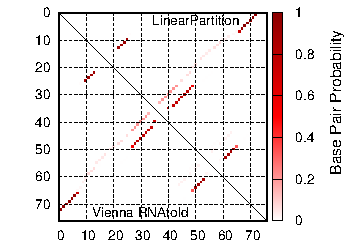
\includegraphics[width=0.33\textwidth]{figs/tRNA_identical_heatmap}
&
% \hspace{-0.8cm}{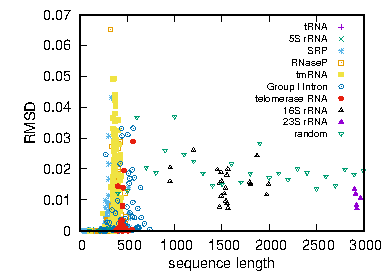
\includegraphics[width=0.33\textwidth]{figs/rmsd_family_plus_random_b2}}
\hspace{-1.1cm}{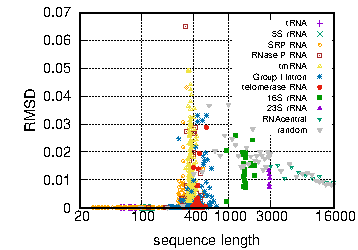
\includegraphics[width=0.33\textwidth]{figs/rmsd_archiveII_rnacentral_lpv_float_plus_long_random}}
% \\[-0.2cm]
&
% \panel{C} & \panel{D}\\[-0.5cm]
\hspace{0.2cm}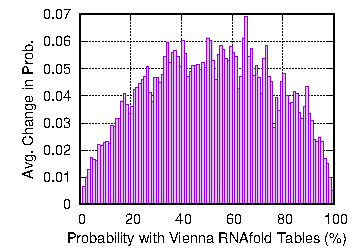
\includegraphics[width=0.33\textwidth]{figs/overall_average_change_prob} \\[-0.1cm]

\hspace{-5.5cm}\panel{C} & \hspace{-6.cm}\panel{D} & \hspace{-5.2cm}\panel{F} \\[-0.5cm]
\hspace{-.8cm}\raisebox{-0.2cm}{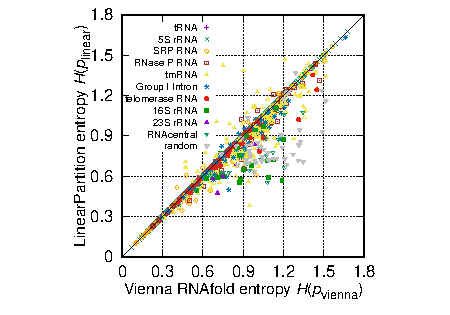
\includegraphics[width=0.35\textwidth]{figs/structure_entropy_xy_plus_random_rnacentral}}
&
\hspace{-0.7cm}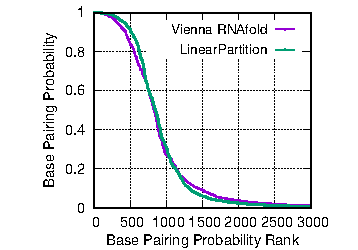
\includegraphics[width=0.33\textwidth]{figs/sorted_prob_23s} 
&
\hspace{-0.0cm}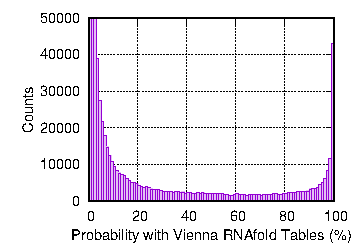
\includegraphics[width=0.34\textwidth]{figs/overall_vienna_prob_bin_count}  \\[-0.2cm]
\end{tabular}
\caption{
Comparison of base pairing probabilities from \viennarnafold and \linearpartition.
	{\bf A}: \linearpartition (upper triangle) and Vienna RNAfold (lower triangle) result in identical base pairing probability matrix for \ecoli tRNA$^\textit{Gly}$.
	{\bf B}: The root-mean-square deviation, $\RMSD(p_\vienna, p_\linear)$, is relatively small between \linearpartition and Vienna RNAfold; all tRNA and 5S rRNA sequences \RMSD is close to 0 (e.g., RMSD$<10^{-5}$).
	{\bf C}: Average positional structural entropy $H(p)$ comparison; \linearpartition has noticeably lower entropy.
	{\bf D}: \linearpartition starts higher and finishes lower than \viennarnafold in a sorted probability curve for \ecoli 23S rRNA,
        suggesting lower entropy.
	{\bf E}: Mean absolute value of change in base pairing probabilities between \viennarnafold and \linearpartition; these changes are averaged within every probability bin.
	{\bf F}: Pair probability distribution of \viennarnafold. 
	Note that the y-axis is limited to 50,000 counts, and the counts of first three bins (with probability smaller than 3\%) are far beyond 50,000.
	\label{fig:rmsd}
}
\vspace{-0.3cm}
\end{figure*}
\fi
